% !TeX program = PdfLaTeX
% !TeX root = ../../Elaborati_Aerodinamica_Bruno_Spoti.tex
\chapter{Aerodinamica viscosa alle alte incidenze}
In questo capitolo saranno svolti calcoli viscosi in condizioni di alta portanza considerando un $Re=1\times10^6$.
Dalla curva di portanza in figura~\vref{fig:cla11} si vede che per questo valore di $Re$ $ {\alpha}_{stall}=13^\circ$. In questa sede si utilizzerà un  {\bfseries $\alpha=12^\circ$} per meglio visualizzare i fenomeni legati alla viscositá.\\ 
In primo luogo sarà graficata la distribuzione del $C_p$ all’angolo di alta portanza scelto. Successivamente saranno analizzati i parametri di strato limite, in termini di H, ${\delta^*}$, ${\theta}$ e $C_f$ in condizioni di piccoli angoli d’attacco e in condizioni di alta portanza. Saranno poi analizzati gli effetti della turbolenza asintotica e della transizione forzata. Infine sarà valutato lo stallo del profilo secondo il criterio semiempirico di Thain e Gault al variare del numero di Reynolds.
\section{Coefficiente di pressione}
\begin{figure} [H]
\centering
\begin{tikzpicture} 
\begin{axis} [ 
ylabel style={rotate=-90}, xmin=0, 
xmax=1, 
ymin=-10,
ymax=2,
xlabel=$\frac{x}{c}$, 
ylabel=$C_p$ ,
 y dir=reverse,
width=12cm,
height=5 cm,
scale only axis,
grid=major] 
\addplot [black,thick, smooth]
file{images/fileDat/EffettiViscosiAlteIncidenze/Cp_alfa_12_Re_1_10e6dorso.dat};
\addplot [black,thick, smooth, dashed]
file{images/fileDat/EffettiViscosiAlteIncidenze/Cp_alfa_12_Re_1_10e6ventre.dat};
\addplot [black,thin,smooth]
file{images/fileDat/EffettiViscosiAlteIncidenze/Cp_alfa_4_Re_1_10e6dorso.dat};
\addplot [black,thin, smooth, dashed]
file{images/fileDat/EffettiViscosiAlteIncidenze/Cp_alfa_4_Re_1_10e6ventre.dat};
\legend {$ \alpha=12^\circ$,$ \alpha=4^\circ$}
\end{axis}
\end{tikzpicture}
\caption{\footnotesize Profilo alare PW106, confronto del coefficiente di pressione $ \alpha=12^\circ$,$ \alpha=4^\circ$. $Re=1\times10^6$. XFOIL 6.99}
\end{figure}

\section{Sviluppo e Parametri di strato limite}
Tramite XFOIL è stato valutato come si sviluppa lo strato limite ad aumentare dell’angolo d’attacco dalle basse incidenze fino ad oltre lo stallo.\\ 
Si nota che all'aumentare del numero di Reynolds la zona di flusso separato sul dorso del profilo si espande sempre più  verso il bordo d'attacco.
\begin{figure}[H]
\centering
\subfloat[][$\alpha=4^\circ$]
{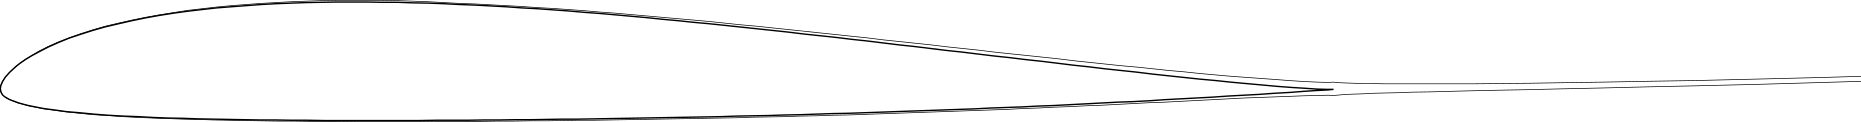
\includegraphics[width=.95\textwidth]{images/fileImg/alfa4_Re_1e6.png}} \\
\subfloat[][$\alpha=12^\circ$]
{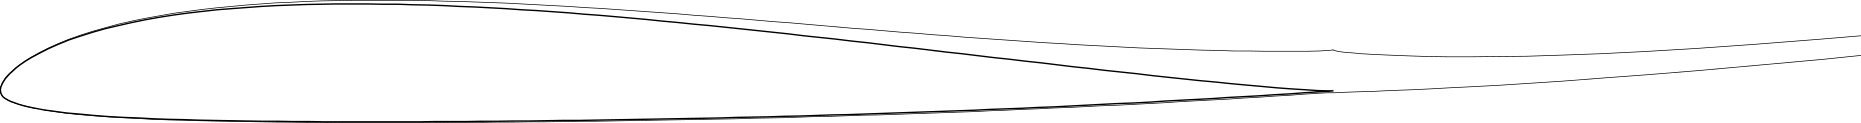
\includegraphics[width=.95\textwidth]{images/fileImg/alfa12_Re_1e6.png}} \\
\subfloat[][$\alpha=19^\circ$]
{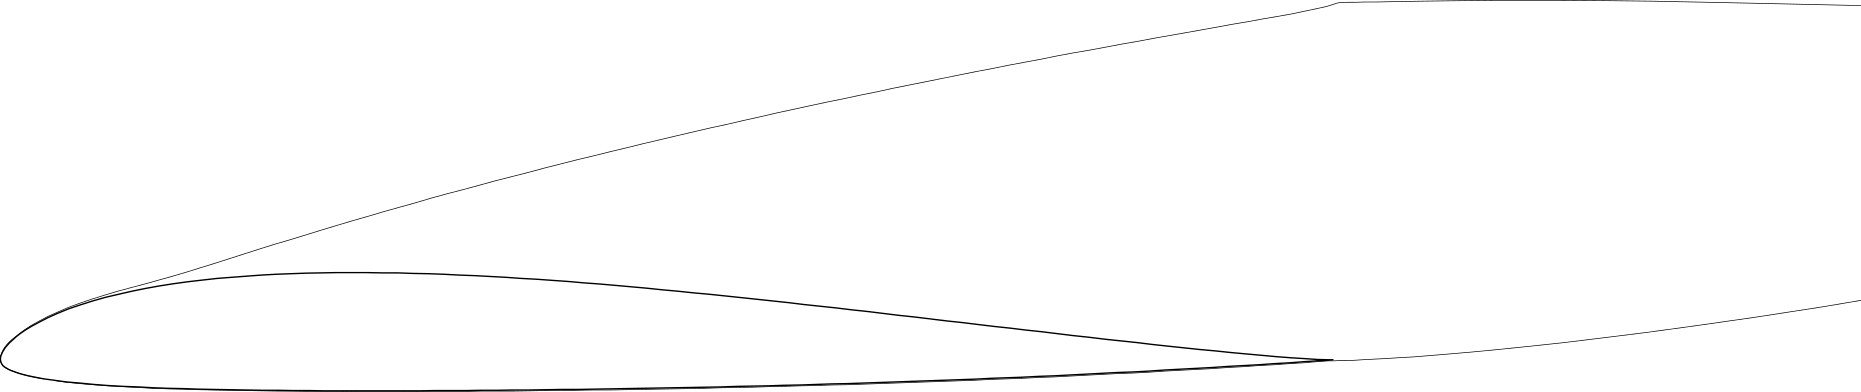
\includegraphics[width=.95\textwidth]{images/fileImg/alfa19_Re_1e6.png}} 
\caption{\footnotesize Profilo PW106, sviluppo dello strato limite, $Re=1\times10^6$, $n_{cr}$=9, transizione libera. XFOIL 6.99}
\label{fig:subfig2}
\end{figure}

Lo strato limite è univocamente definito assegnata la terna H, ${\delta^*}$, ${\theta}$. Di seguito sará studiata la variazione di questi parametri con l’angolo d’attacco congiuntamente allo studio della variazione del coefficiente d’attrito.\\
Si noti che sul ventre del profilo a nessuna incidenza si verificano particolari fenomeni di separazione e il flusso resta laminare.

\begin{figure} [H]
\centering
\begin{tikzpicture} 
\begin{axis} [ 
ylabel style={rotate=-90}, xmin=0, 
xmax=2.02, 
ymin=0,
ymax=10,
xlabel=$\frac{s}{c}$,
ylabel=$H$ ,
width=12cm,
height=8.5 cm,
scale only axis,
grid=major] 
\addplot [black,very thin,smooth]
file{images/fileDat/EffettiViscosiAlteIncidenze/H_alfa4_Re_1e6.dat};
\addplot [black,very thick, smooth]
file{images/fileDat/EffettiViscosiAlteIncidenze/H_alfa12_Re_1e6.dat};
\legend { $ \alpha=4^\circ$,$ \alpha=12^\circ$}
\end{axis}
\end{tikzpicture}
\caption{\footnotesize Profilo alare PW106, confronto dell'andamento del fattore di forma H al variare dell'angolo d'attacco. XFOIL 6.99}
\end{figure}
\noindent


\begin{figure} [H]
\centering
\begin{tikzpicture} 
\begin{axis} [ 
ylabel style={rotate=-90}, xmin=0, 
xmax=2.02, 
ymin=-0.01,
ymax=0.1,
xlabel=$\frac{s}{c}$,
ylabel=$C_f$ ,
width=12cm,
height=8.5 cm,
scale only axis,
grid=major] 
\addplot [black,very thin,smooth]
file{images/fileDat/EffettiViscosiAlteIncidenze/Cf_alfa4_Re_1e6.dat};
\addplot [black,very thick, smooth]
file{images/fileDat/EffettiViscosiAlteIncidenze/Cf_alfa12_Re_1e6.dat};;
\legend { $ \alpha=4^\circ$,$ \alpha=12^\circ$}
\end{axis}
\end{tikzpicture}
\caption{\footnotesize Profilo alare PW106, confronto dell'andamento del Coefficiente d'attrito $C_f$ al variare dell'angolo d'attacco. XFOIL 6.99}
\end{figure}
\noindent \\ \\ 

Il particolare andamento del coefficiente d'attrito e del fattore di forma per $ \alpha=12^\circ$ è deducibile da un’analisi dello sviluppo dello strato limite alle alte incidenze. Nel punto di ristagno anteriore la velocità locale è nulla, quindi sarà nullo anche il numero di Reynolds locale, calcolato rispetto la distanza dal {\itshape nose}. Ciò vuol dire che ivi le $\tau$ sono molto alte e, pertanto, sono in grado di annichilire ogni disturbo. In questo punto si avrà, quindi, un $C_f$ molto alto e un H piuttosto basso. Procedendo verso il TE sul dorso si incontra una bolla laminare alla quale corrisponde un intervallo di $C_f$ negativi e un picco nel fattore di forma. La bolla comporta una separazione laminare, ma anche la transizione a turbolento che energizza il flusso e consente il riattacco con un conseguente aumento di $C_f$. Si ha così un flusso turbolento attaccato più energizzato, che porta ad una diminuzione di H. L'alta incidenza non consente di avere un flusso attaccato per un ampio intervallo di profilo e quindi separa, facendo si che H cresca fino al TE.

\begin{figure} [H]
\centering
\begin{tikzpicture} 
\begin{axis} [ 
ylabel style={rotate=-90}, xmin=0, 
xmax=2.02, 
ymin=-0.01,
ymax=0.015,
xlabel=$\frac{s}{c}$,
ylabel= ${\theta}$ ,
width=0.9\textwidth,
height=6cm,
scale only axis,
grid=major] 
\addplot [black,very thin,smooth]
file{images/fileDat/EffettiViscosiAlteIncidenze/Theta_alfa4_Re_1e6.dat};
\addplot [black,very thick, smooth]
file{images/fileDat/EffettiViscosiAlteIncidenze/Theta_alfa12_Re_1e6.dat};;
\legend { $ \alpha=4^\circ$,$ \alpha=12^\circ$}
\end{axis}
\end{tikzpicture}
\caption{\footnotesize Profilo alare PW106, confronto dell'andamento dello spessore di quantità di moto  ${\theta}$ al variare dell'angolo d'attacco. XFOIL 6.99}
\end{figure}
\begin{figure} [H]
\centering
\begin{tikzpicture} 
\begin{axis} [ 
ylabel style={rotate=-90}, xmin=0, 
xmax=2.02, 
ymin=-0.01,
ymax=0.05,
xlabel=$\frac{s}{c}$, 
ylabel=${\delta^*}$ ,
width=0.9\textwidth,
height=6cm,
scale only axis,
grid=major] 
\addplot [black,very thin,smooth]
file{images/fileDat/EffettiViscosiAlteIncidenze/Delta_star_alfa4_Re_1e6.dat};
\addplot [black,very thick, smooth]
file{images/fileDat/EffettiViscosiAlteIncidenze/Delta_star_alfa12_Re_1e6.dat};;
\legend { $ \alpha=4^\circ$,$ \alpha=12^\circ$}
\end{axis}
\end{tikzpicture}
\caption{\footnotesize Profilo alare PW106, confronto dell'andamento dello spessore di spostamento ${\delta^*}$ al variare dell'angolo d'attacco. XFOIL 6.99}
\end{figure}
\noindent \\ \\ 



\section{Effetto della variazione del numero di Reynolds e stallo}

Da uno zoom sul grafico della curva di portanza, si può notare come il $C_{l_\mathrm{max}}$ cresce all'aumentare del numero di Reynolds con un conseguente aumento dell'${\alpha}_{stall}$
Nella tabella \ref{tab:rei} sono riportati i valori dell'angolo di stallo e del $C_{l_\mathrm{max}}$ a vari numeri di Reynolds.

\begin{table}[htbp]\centering \rowcolors{1}{}{grigio_chiaro}
\begin{tabular}{c S c c}
\toprule
\emph{Numero di Reynolds} & $ C_{l_\mathrm{max}}$  & ${\alpha}_\mathrm{stall}$  \\
\midrule
$5\times10^5$ & 1.28 & $13^\circ$ \\
$1\times10^6$ & 1.38 & $13^\circ$ \\
$3\times10^6 $ & 1.56 & $16^\circ$ \\
$1\times10^7 $& 1.76 & $18^\circ$ \\
\bottomrule
\end{tabular}
\caption {$C_{l_\mathrm{max}}$ e ${\alpha}_\mathrm{stall}$ al variare del numero di Reynolds}
\label{tab:rei}
\end{table}
\begin{figure} [H]
\centering
\begin{tikzpicture} 
\begin{axis} [ 
legend style={at={(0.45,0.98)}},
ylabel style={rotate=-90}, xmin=8, 
xmax=25, 
ymin=1,
ymax=2,
xlabel=${\alpha}$,
ylabel=$C_l$ ,
width=8cm,
height=9.5 cm,
scale only axis,
grid=major] 
\addplot [black, smooth,mark=*]
file{images/fileDat/EffettiViscosi/Cl_vs_alpha_Re_5_10_5.dat};
\addplot [black,smooth,mark=square]
file{images/fileDat/EffettiViscosi/Cl_vs_alpha_Re_1_10_6.dat};
\addplot [black, smooth,mark=diamond*]
file{images/fileDat/EffettiViscosi/Cl_vs_alpha_Re_3_10_6.dat};
\addplot [black, smooth,mark=star]
file{images/fileDat/EffettiViscosi/Cl_vs_alpha_Re_1_10_7.dat};
\legend {$Re=5\times10^5  $,$Re=1\times10^6$,$Re=3\times10^6$,$Re=1\times10^7$}
\end{axis}
\end{tikzpicture} 
\caption{\footnotesize Confronto delle curve di Portanza del profilo PW106 a vari numeri di Reynolds, zoom della zona di stallo. XFOIL 6.99}
\label{fig:cla2}
\end{figure}



Di seguito sarà analizzato l'andamento del $C_p$ allo stallo per diversi numeri di Reynolds al fine di vedere che tipo di stallo interessa il profilo in date condizioni.

\begin{figure} [H]
\centering
\begin{tikzpicture} 
\begin{axis} [ 
ylabel style={rotate=-90}, xmin=0, 
xmax=1, 
ymin=-17,
ymax=1.2,
xlabel=$\frac{x}{c}$, 
ylabel=$C_p$ ,
 y dir=reverse,
width=13cm,
height=7cm,
scale only axis,
grid=major] 
\addplot [black,very thick]
file{images/fileDat/EffettiViscosiAlteIncidenze/Cp_stall_Re5e5dorso.dat};
\addplot [black, semithick]
file{images/fileDat/EffettiViscosiAlteIncidenze/Cp_stall_Re1e6dorso.dat};
\addplot [black, thin]
file{images/fileDat/EffettiViscosiAlteIncidenze/Cp_stall_Re1e7dorso.dat};
\addplot [black,very thick, dashed]
file{images/fileDat/EffettiViscosiAlteIncidenze/Cp_stall_Re5e5ventre.dat};
\addplot [black, semithick, dashed]
file{images/fileDat/EffettiViscosiAlteIncidenze/Cp_stall_Re1e6ventre.dat};
\addplot [black, thin, dashed]
file{images/fileDat/EffettiViscosiAlteIncidenze/Cp_stall_Re1e7ventre.dat};
\legend {$Re=5\times10^5$,$Re=1\times10^6$,$Re=10\times10^6$}
\end{axis}
\end{tikzpicture}
\caption{\footnotesize Profilo alare PW106, confronto del coefficiente di pressione allo stallo sul dorso del profilo (linea continua) e sul ventre (linea tratteggiata) a diversi valori numero di Reynolds. XFOIL 6.99 }\label{fig:stall}
\end{figure}
\noindent \\


\begin{figure} [H]
\centering
\begin{tikzpicture} 
\begin{axis} [ 
ylabel style={rotate=-90}, xmin=0, 
xmax=0.05, 
ymin=-10,
ymax=-6,
xlabel=$\frac{x}{c}$, 
ylabel=$C_p$ ,
 y dir=reverse,
width=10cm,
height=6cm,
scale only axis,
grid=major] 
\addplot [black,very thick]
file{images/fileDat/EffettiViscosiAlteIncidenze/Cp_stall_Re5e5dorso.dat};
\addplot [black, semithick]
file{images/fileDat/EffettiViscosiAlteIncidenze/Cp_stall_Re1e6dorso.dat};
\addplot [black, thin]
file{images/fileDat/EffettiViscosiAlteIncidenze/Cp_stall_Re1e7dorso.dat};
\addplot [black,very thick, dashed]
file{images/fileDat/EffettiViscosiAlteIncidenze/Cp_stall_Re5e5ventre.dat};
\addplot [black, semithick, dashed]
file{images/fileDat/EffettiViscosiAlteIncidenze/Cp_stall_Re1e6ventre.dat};
\addplot [black, thin, dashed]
file{images/fileDat/EffettiViscosiAlteIncidenze/Cp_stall_Re1e7ventre.dat};
\legend {$Re=5\times10^5$,$Re=1\times10^6$,$Re=10\times10^6$}
\end{axis}
\end{tikzpicture}
\caption{\footnotesize Profilo alare PW106, zoom del particolare nel confronto del coefficiente di pressione allo stallo a diversi valori numero di Reynolds. XFOIL 6.99}\label{fig:stallz}
\end{figure}
\noindent \\


Dalle figure  \ref{fig:stall} e  \ref{fig:stallz} si può notare il diverso comportamento del profilo in condizioni di stallo al variare del numero di Reynolds. \\Per $Re=5\times10^5$ si può osservare la formazione di una bolla laminare sul dorso del profilo, verso il LE. %Tale bolla ha un’estensione di circa il $20\%$ della corda.
Ciò può essere confermato dall’intervallo di valori negativi del coefficiente di attrito diagrammati in figura \ref{fig:coef} cui corrisponde un picco nel diagramma di H come si vede in figura \ref{fig:h}.
Per $Re=1\times10^6$ si ha una bolla più corta che potrebbe esser causa di uno stallo da esplosione da bolla, più violento. Aumentando il numero di Reynolds, fino ad un valore di $Re=10\times10^6$ la bolla scompare cosicché il profilo è caratterizzato da uno stallo turbolento.\\
È possibile verificare queste considerazioni nei grafici  riportati in figura~\vref{fig:h} e~\vref{fig:coef} che esprimono i parametri di strato limite più significativi in tal senso. Alla presenza di una bolla corrispondono zone di $C_f$  negative piú o meno estese e picchi nel fattore di forma H.
%
%\noindent \\  \\



\begin{figure} [H]
\centering
\begin{tikzpicture} 
\begin{axis} [ 
ylabel style={rotate=-90}, xmin=0, 
xmax=2.02, 
ymin=0,
ymax=13,
xlabel=$\frac{s}{c}$,
ylabel=$H$ ,
width=12cm,
height=9 cm,
scale only axis,
grid=major] 
\addplot [black,very thick]
file{images/fileDat/EffettiViscosiAlteIncidenze/H_stall_Re5e5.dat};
\addplot [black, semithick]
file{images/fileDat/EffettiViscosiAlteIncidenze/H_stall_Re1e6.dat};
\addplot [black, very thin]
file{images/fileDat/EffettiViscosiAlteIncidenze/H_stall_Re1e7.dat};
\legend {$Re=5\times10^5$,$Re=1\times10^6$,$Re=10\times10^6$}
\end{axis}
\end{tikzpicture}
\caption{\footnotesize Profilo alare PW106, confronto dell'andamento del fattore di forma H allo stallo al variare del numero di Reynolds. XFOIL 6.99}
\label{fig:h}
\end{figure}
\noindent


\begin{figure} [H]
\centering
\begin{tikzpicture} 
\begin{axis} [ 
ylabel style={rotate=-90}, xmin=0, 
xmax=2.02, 
ymin=-0.01,
ymax=0.14,
xlabel=$\frac{s}{c}$,
ylabel=$C_f$ ,
width=12cm,
height=7cm,
scale only axis,
grid=major] 
\addplot [black,very thick]
file{images/fileDat/EffettiViscosiAlteIncidenze/Cf_stall_Re5e5.dat};
\addplot [black, semithick]
file{images/fileDat/EffettiViscosiAlteIncidenze/Cf_stall_Re1e6.dat};
\addplot [black, very thin]
file{images/fileDat/EffettiViscosiAlteIncidenze/Cf_stall_Re1e7.dat};
\legend {$Re=5\times10^5$,$Re=1\times10^6$,$Re=10\times10^6$}
\end{axis}
\end{tikzpicture}
\caption{\footnotesize Profilo alare PW106, confronto dell'andamento del coefficiente d'attrito $C_f$ allo stallo al variare del numero di Reynolds. XFOIL 6.99}
\label{fig:coef}
\end{figure}
 \noindent \\ 


Questi risultati sono confermati dal criterio semiempirico di stallo di Thain e Gault.\\
 Per verificare il tipo di stallo è stato calcolato lo spessore percentuale del profilo ad ${\frac {x}{c} }=0.0125$ ottenendo un valore di $1.75 \%$ entrando, in tal modo, nel grafico riportato in figura~\vref{fig:tin}.



\begin {figure} [H]
\centering
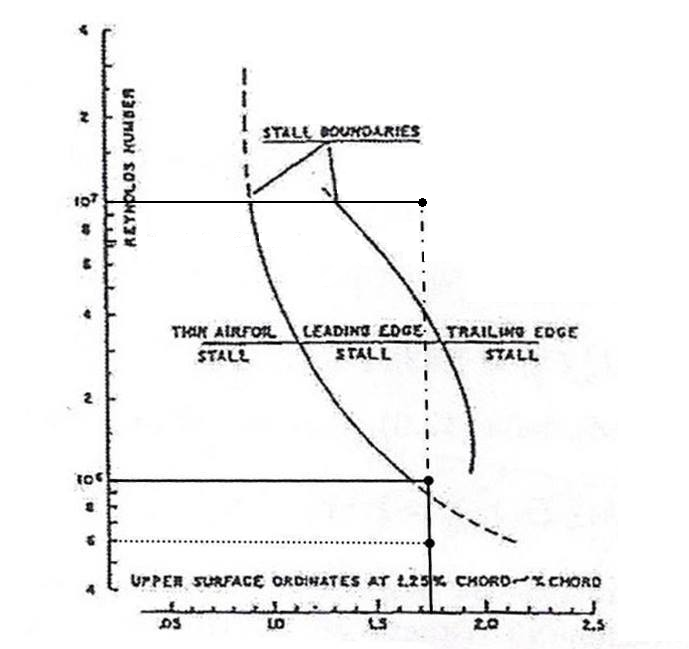
\includegraphics[width= 12cm ]{images/fileImg/thin.png}
\caption{\footnotesize Criterio di Thain e Gault, risultati per il profilo PW106}
\label {fig:tin}
\end {figure}
